To study the efficiency of Lazy Shadowing in terms of reliability, completion time, and energy consumption, we compare with traditional process replication using the analytical models developed in Section~\ref{sec:analytical}. We also compare to checkpointing, of which the completion time is calculated with Daly's model~\cite{daly_fgcs_2006} assuming the recovery time and checkpointing time are both 10 minutes, and then the energy consumption is derived using Equation~\ref{eq:exp_energy1}. 
It is clear from Equation~\ref{eq:time_k} that the total recovery delay $\sum_{i=1}^k\tau_i$ is determined by the execution time $\sum_{i=1}^k\Delta_i$, independent of the distribution of failures which determines 
the individual value of $\Delta_i$. 
Therefore, our models are generic with no assumption about failure probability distribution, and the expectation of the total delay from all failures is the same as the failures are uniformly distributed~\cite{daly_fgcs_2006}. Specifically, $\Delta_i = w/(k+1)$, and $T_c^k$ can be rewritten as $w + w*(1-\sigma_s^b)*\frac{k}{k+1}$ for Lazy Shadowing. Further, we assume that each shadow process gets a fair share of its shadow core's execution rate so that $\sigma_s^b = \frac{1}{\alpha}$. One may argue that the execution rate of the shadows
should be degraded because of increased memory pressure or communication overhead. %Agreeing with that, however, we argue that 
%time sharing, which is the basic mechanism of multi-programming OS, is able to overlap computation and communication and improve system efficiency. For completeness, though, 
To take that into account, we have also studied the slowing down effect using a penalty model, to be discussed later. 
To calculate the expected energy consumption for Lazy Shadowing with Equation~\ref{eq:exp_energy2}, we further assume that the dynamic power during shadow leaping is twice that during normal execution, i.e., $p_{l}=2*p_d$, and the time for shadow leaping through RDMA is half of the time required for recovery, i.e., $T_l=0.5*(T_{total} - w)$. The static power ratio $\rho$ is fixed at 0.5 for now, other values will be explored later in this section.

The first study uses $N=1$ million cores, effectively simulating the future extreme-scale computing environment, and assumes that $W=1$ million hours. 
For Lazy Shadowing we varied $\alpha$ from 1 to 10, with the understanding that it is unrealistic to collocate too many processes on a core. Besides $\alpha=1$, which is equivalent to process replication, we only show $\alpha=5$ and $\alpha=10$ as others can be easily inferred from the figures.

\begin{figure}[!t]
	\begin{center}
		\subfigure[Application failure probability]
		{
			\label{fig:f3}
			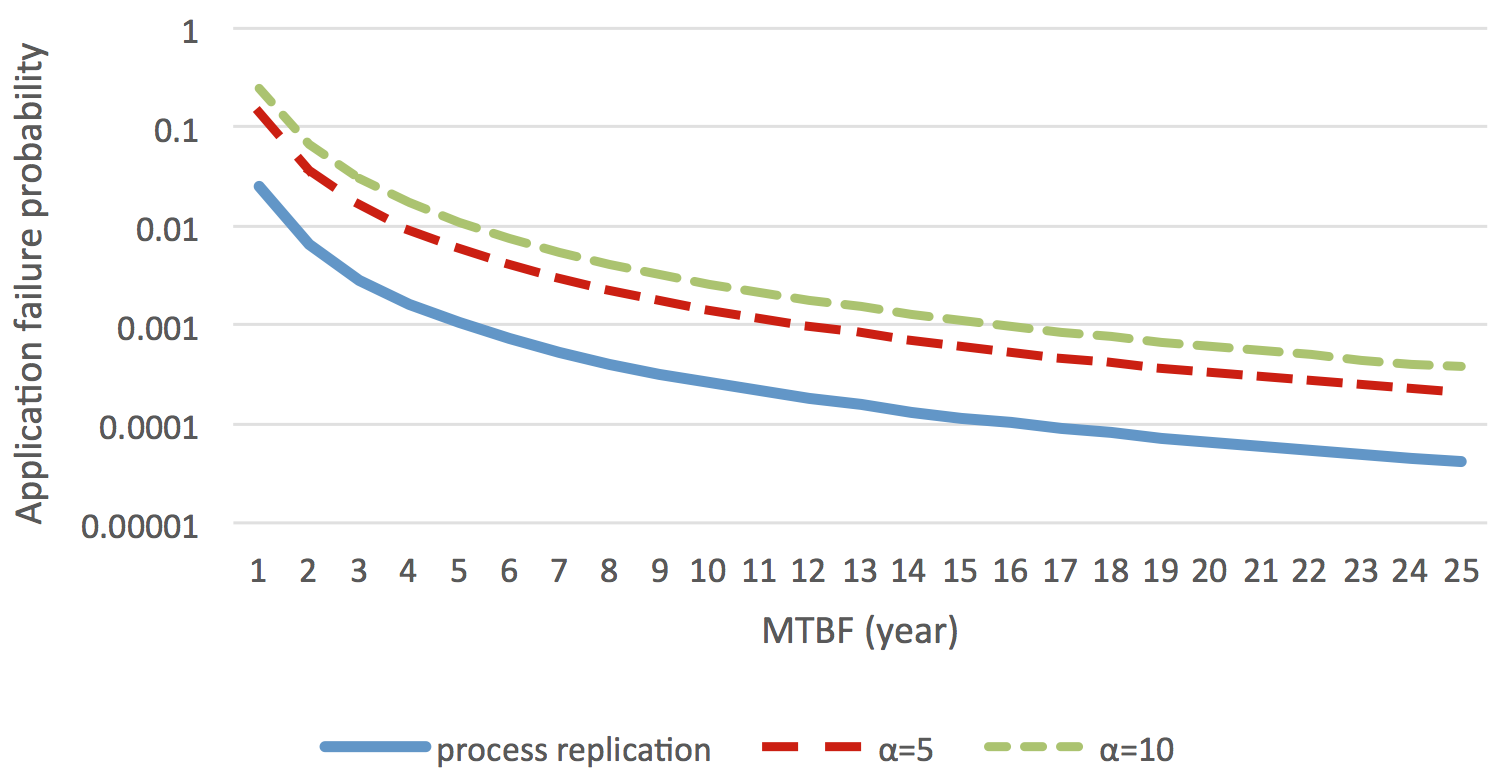
\includegraphics[width=0.8\columnwidth]{Figures/f3}
		} 
		\subfigure[Expected completion time]
		{
			\label{fig:t31}
			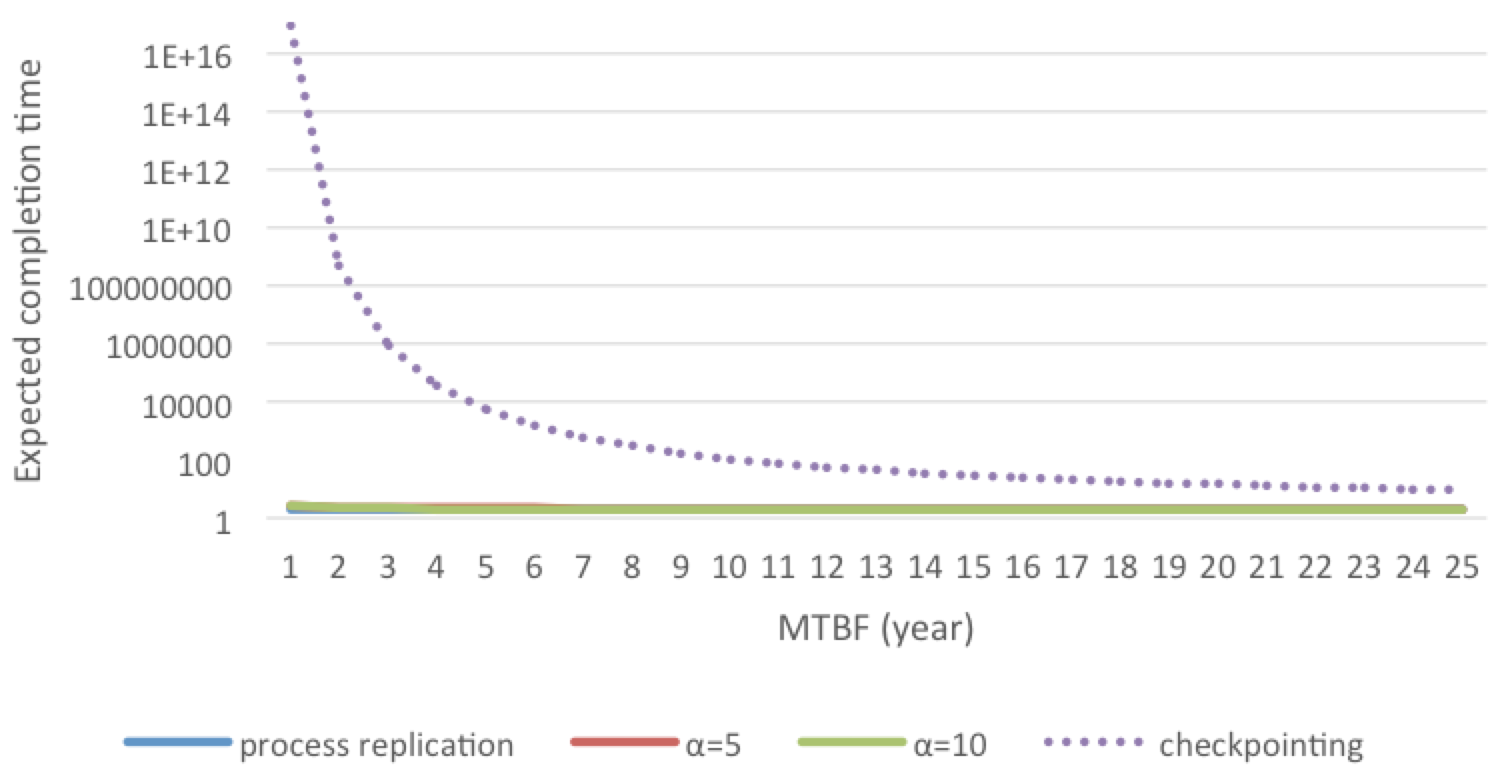
\includegraphics[width=0.8\columnwidth]{Figures/t31}
		} 
		\subfigure[Expected completion time with checkpointing removed]
		{
			\label{fig:t32}
			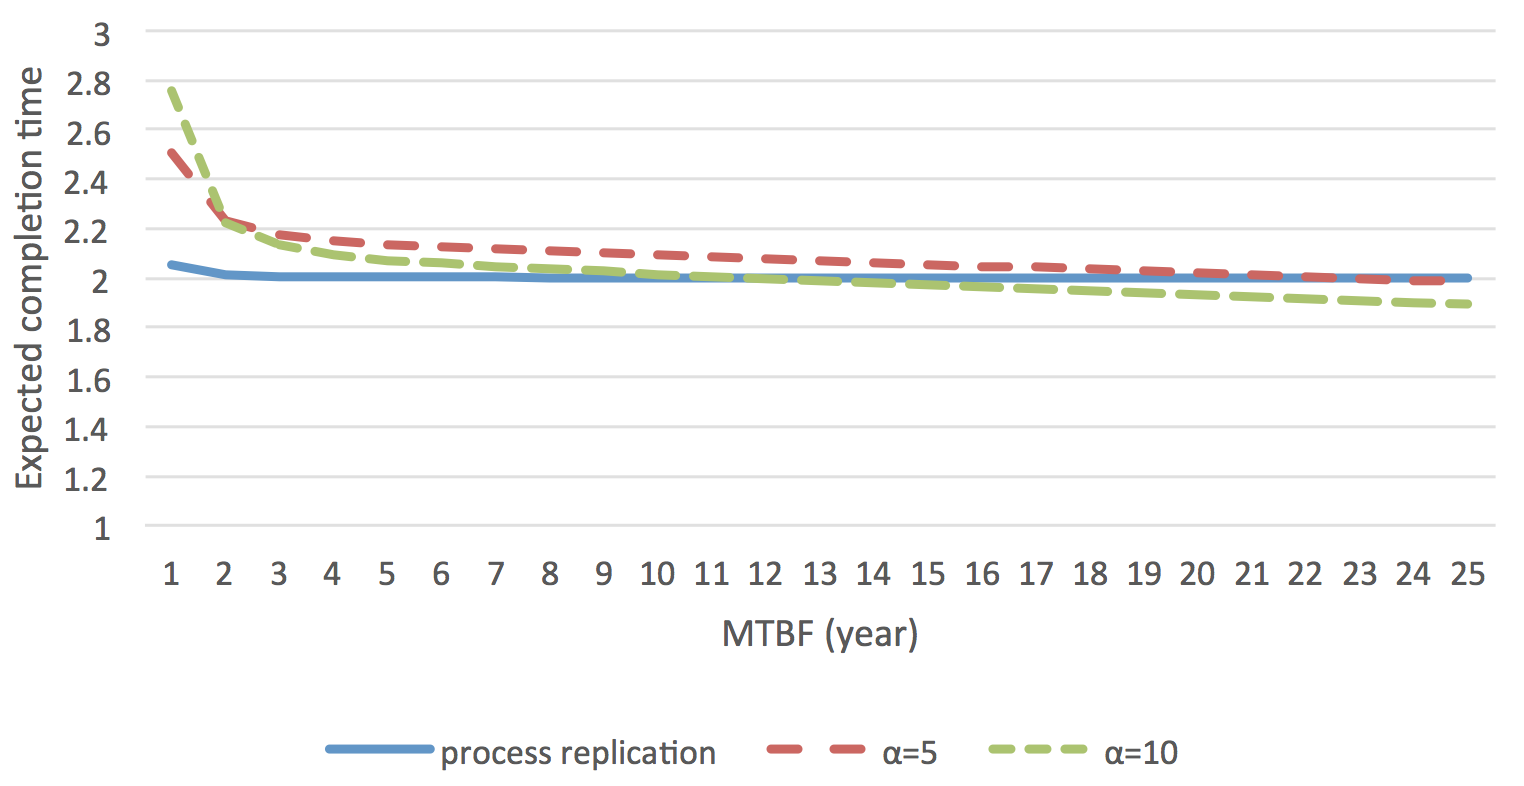
\includegraphics[width=0.8\columnwidth]{Figures/t32}
		} 
		\subfigure[Expected energy consumption with checkpoting removed]
		{
			\label{fig:e32}
			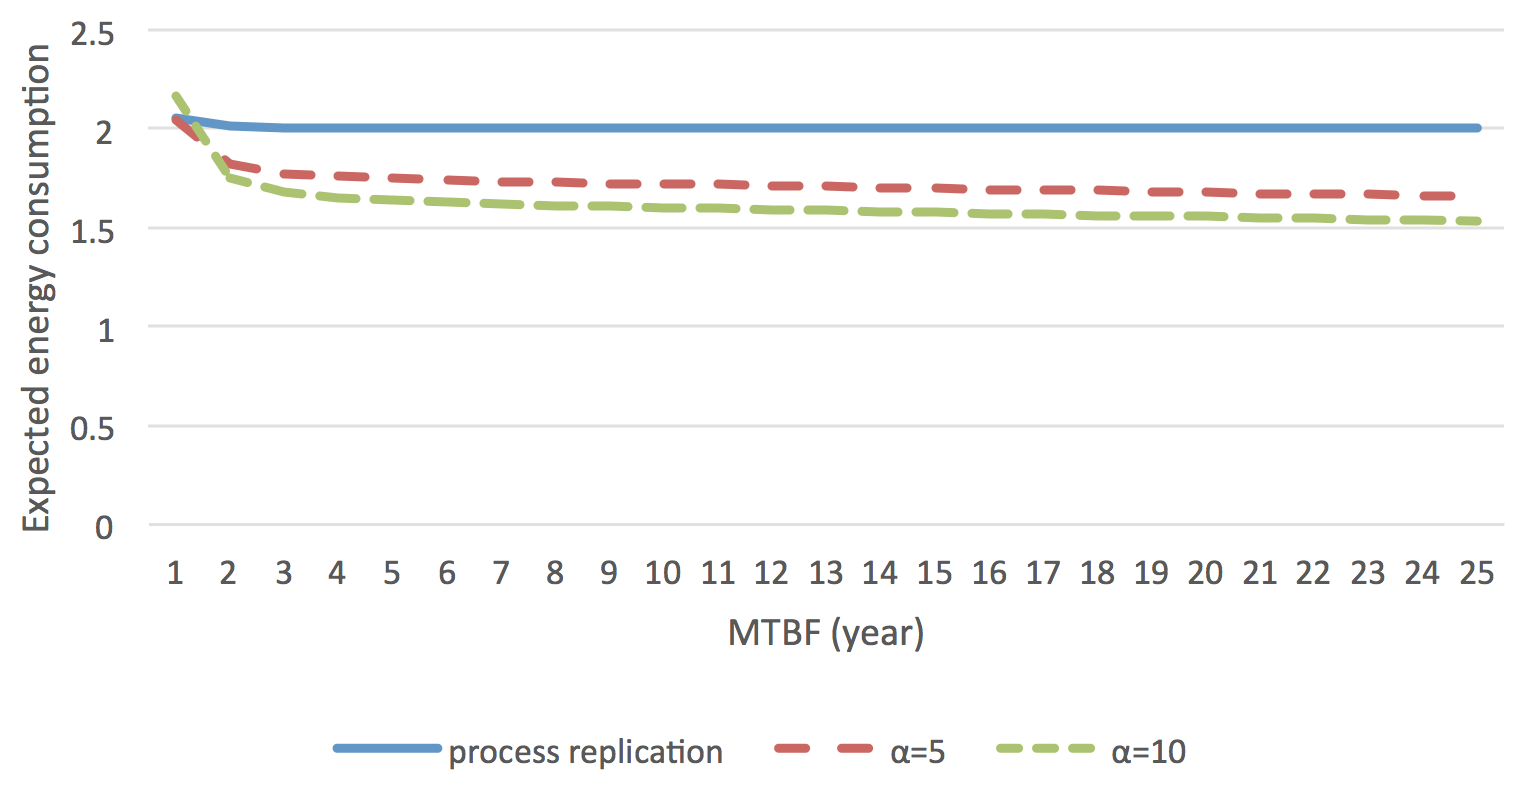
\includegraphics[width=0.8\columnwidth]{Figures/e32}
		} 
	\end{center}
	%\vskip -0.22in 
	\caption{Comparision to process replication and checkpointing. $W=10^6$ hours, $N=10^6$, $\rho=0.5$.}
	\label{fig:3}
\end{figure}

By definition, the application failure probability for checkpointing is 0, as it periodically saves the execution states, from which the computation can be resumed upon failure. Figure~\ref{fig:f3} shows that due to collocation, the application failure probability increases for Lazy Shadowing. However, even with the lowest MTBF (1 year), Lazy Shadowing is still able to complete the application without re-execution with larger than 0.75 probability. 

It is clear from Figure~\ref{fig:t31} that checkpointing incurs significant delay, indicating that it may not be a viable fault tolerance approach for future extreme-scale computing. The completion time and energy consumption of checkpointing are so large that the comparison between process replication and Lazy Shadowing is invisible. Therefore, we re-plot the comparison between Lazy Shadowing and process replication in Figure~\ref{fig:t32} and~\ref{fig:e32}, with checkpointing removed. Figure~\ref{fig:t32} reveals that the most time efficient choice depends on MTBF. More specifically, process replication is more suited when MTBF is low while otherwise Lazy Shadowing is better. In terms of energy consumption, the advantage of Lazy Shadowing is much more obvious. For MTBF from 2 to 25 years, Lazy Shadowing with $\alpha=5$ can achieve 9.6-17.1\% energy saving, while the saving increases to 13.1- 23.3\% for $\alpha=10$. The only exception is when MTBF is extremely low (1 year), Lazy Shadowing with $\alpha=10$ consumes more energy than process replication because of its higher probability of re-execution.






